\documentclass[a4paper, 14pt, oneside,openany]{memoir}

%%% Задаем поля, отступы и межстрочный интервал %%%

\usepackage[left=30mm, right=15mm, top=20mm, bottom=20mm]{geometry} % Пакет geometry с аргументами для определения полей
\pagestyle{plain} % Убираем стандарные для данного класса верхние колонтитулы с заголовком текущей главы, оставляем только номер страницы снизу по центру
\parindent=1.25cm % Абзацный отступ 1.25 см, приблизительно равно пяти знакам, как по ГОСТ
\usepackage{indentfirst} % Добавляем отступ к первому абзацу
%\linespread{1.3} % Межстрочный интервал (наиболее близко к вордовскому полуторному) - тут вместо этого используется команда OnehalfSpacing*

%%% Работаем с URL
\usepackage{xurl}


%%% Задаем языковые параметры и шрифт %%%
\usepackage{graphicx}
\usepackage{verbatim}
\usepackage{float}
\usepackage{xcolor}
\usepackage{mdframed}
\usepackage[shortlabels]{enumitem}
\usepackage{indentfirst}
\usepackage{hyperref}

%%% Оформление алгоритмов и псевдокда %%%
\usepackage{algorithm}
\usepackage{algpseudocode}



\usepackage[english, russian]{babel}                % Настройки для русского языка как основного в тексте
\usepackage[T2A]{fontenc}
% \babelfont{rm}{Times New Roman}                     % TMR в качестве базового roman-щрифта

%%% Задаем стиль заголовков и подзаголовков в тексте %%%

\setsecnumdepth{subsection} % Номера разделов считать до третьего уровня включительно, т.е. нумеруются только главы, секции, подсекции
\renewcommand*{\chapterheadstart}{} % Переопределяем команду, задающую отступ над заголовком, чтобы отступа не было
\renewcommand*{\printchaptername}{} % Переопределяем команду, печатающую слово "Глава", чтобы оно не печалось
%\renewcommand*{\printchapternum}{} % То же самое для номера главы - тут не надо, номер главы оставляем
\renewcommand*{\chapnumfont}{\normalfont\bfseries} % Меняем стиль шрифта для номера главы: нормальный размер, полужирный
\renewcommand*{\afterchapternum}{\hspace{1em}} % Меняем разделитель между номером главы и названием
\renewcommand*{\printchaptertitle}{\normalfont\bfseries\centering\MakeUppercase} % Меняем стиль написания для заголовка главы: нормальный размер, полужирный, центрированный, заглавными буквами
\setbeforesecskip{20pt} % Задаем отступ перед заголовком секции
\setaftersecskip{20pt} % Ставим такой же отступ после заголовка секции
\setsecheadstyle{\raggedright\normalfont\bfseries} % Меняем стиль написания для заголовка секции: выравнивание по правому краю без переносов, нормальный размер, полужирный
\setbeforesubsecskip{20pt} % Задаем отступ перед заголовком подсекции
\setaftersubsecskip{20pt} % Ставим такой же отступ после заголовка подсекции
\setsubsecheadstyle{\raggedright\normalfont\bfseries}  % Меняем стиль написания для заголовка подсекции: выравнивание по правому краю без переносов, нормальный размер, полужирный

%%% Задаем параметры оглавления %%%

\addto\captionsrussian{\renewcommand\contentsname{Содержание}} % Меняем слово "Оглавление" на "Содержание"
\setrmarg{2.55em plus1fil} % Запрещаем переносы слов в оглавлении
% \setlength{\cftbeforechapterskip}{0pt} % Эта команда убирает интервал между заголовками глав - тут не надо, так красивее смотрится
\renewcommand{\aftertoctitle}{\afterchaptertitle \vspace{-\cftbeforechapterskip}} % Делаем отступ между словом "Содержание" и первой строкой таким же, как у заголовков глав
%\renewcommand*{\chapternumberline}[1]{} % Делаем так, чтобы номер главы не печатался - тут не надо
\renewcommand*{\cftchapternumwidth}{1.5em} % Ставим подходящий по размеру разделитель между номером главы и самим заголовком
\renewcommand*{\cftchapterfont}{\normalfont\MakeUppercase} % Названия глав обычным шрифтом заглавными буквами
\renewcommand*{\cftchapterpagefont}{\normalfont} % Номера страниц обычным шрифтом
\renewcommand*{\cftchapterdotsep}{\cftdotsep} % Делаем точки до номера страницы после названий глав
\renewcommand*{\cftdotsep}{1} % Задаем расстояние между точками
\renewcommand*{\cftchapterleader}{\cftdotfill{\cftchapterdotsep}} % Делаем точки стандартной формы (по умолчанию они "жирные")
\maxtocdepth{section} % В оглавление попадают только разделы первых двух уровней: главы, секции

\newenvironment{problem}[2][]
    { \begin{mdframed}[backgroundcolor=gray!10] \textbf{#1 #2.} \\}
    {  \end{mdframed}}


% %%% Задаём вид для списков %%%
% \newenvironment{itemlist}[1]{%
%   \begin{trivlist}
%   \item \textbf{\large #1}
%   \begin{itemize}
% }{%
%   \end{itemize}
%   \end{trivlist}
% }


%%% Выравнивание и переносы %%%

%% http://tex.stackexchange.com/questions/241343/what-is-the-meaning-of-fussy-sloppy-emergencystretch-tolerance-hbadness
%% http://www.latex-community.org/forum/viewtopic.php?p=70342#p70342
\tolerance 1414
\hbadness 1414
\emergencystretch 1.5em                             % В случае проблем регулировать в первую очередь
\hfuzz 0.3pt
\vfuzz \hfuzz
%\dbottom
%\sloppy                                            % Избавляемся от переполнений
\clubpenalty=10000                                  % Запрещаем разрыв страницы после первой строки абзаца
\widowpenalty=10000                                 % Запрещаем разрыв страницы после последней строки абзаца
\brokenpenalty=4991                                 % Ограничение на разрыв страницы, если строка заканчивается переносом

%%% Объясняем компилятору, какие буквы русского алфавита можно использовать в перечислениях (подрисунках и нумерованных списках) %%%
%%% По ГОСТ нельзя использовать буквы ё, з, й, о, ч, ь, ы, ъ %%%
%%% Здесь также переопределены заглавные буквы %%%

\makeatletter
    \def\russian@Alph#1{\ifcase#1\or
       А\or Б\or В\or Г\or Д\or Е\or Ж\or
       И\or К\or Л\or М\or Н\or
       П\or Р\or С\or Т\or У\or Ф\or Х\or
       Ц\or Ш\or Щ\or Э\or Ю\or Я\else\xpg@ill@value{#1}{russian@Alph}\fi}
    \def\russian@alph#1{\ifcase#1\or
       а\or б\or в\or г\or д\or е\or ж\or
       и\or к\or л\or м\or н\or
       п\or р\or с\or т\or у\or ф\or х\or
       ц\or ш\or щ\or э\or ю\or я\else\xpg@ill@value{#1}{russian@alph}\fi}
\makeatother

%%% Задаем параметры оформления рисунков и таблиц %%%

\usepackage{graphicx, caption, subcaption} % Подгружаем пакеты для работы с графикой и настройки подписей
\graphicspath{{images/}} % Определяем папку с рисунками
\captionsetup[figure]{font=small, width=\textwidth, name=Рисунок, justification=centering} % Задаем параметры подписей к рисункам: маленький шрифт (в данном случае 12pt), ширина равна ширине текста, полнотекстовая надпись "Рисунок", выравнивание по центру
\captionsetup[subfigure]{font=small} % Индексы подрисунков а), б) и так далее тоже шрифтом 12pt (по умолчанию делает еще меньше)
\captionsetup[table]{singlelinecheck=false,font=small,width=\textwidth,justification=justified} % Задаем параметры подписей к таблицам: запрещаем переносы, маленький шрифт (в данном случае 12pt), ширина равна ширине текста, выравнивание по ширине
\captiondelim{ --- } % Разделителем между номером рисунка/таблицы и текстом в подписи является длинное тире
\setkeys{Gin}{width=\textwidth} % По умолчанию размер всех добавляемых рисунков будет подгоняться под ширину текста
\renewcommand{\thesubfigure}{\asbuk{subfigure}} % Нумерация подрисунков строчными буквами кириллицы
\usepackage[section]{placeins} % Объекты типа float (рисунки/таблицы) не вылезают за границы секциии, в которой они объявлены


%%% Задаем параметры ссылок и гиперссылок %%% 

\usepackage{hyperref}                               % Подгружаем нужный пакет
\hypersetup{
    colorlinks=true,                                % Все ссылки и гиперссылки цветные
    linktoc=all,                                    % В оглавлении ссылки подключатся для всех отображаемых уровней
    linktocpage=true,                               % Ссылка - только номер страницы, а не весь заголовок (так выглядит аккуратнее)
    linkcolor=red,                                  % Цвет ссылок и гиперссылок - красный
    citecolor=red                                   % Цвет цитировний - красный
}

%%% Настраиваем отображение списков %%%

\usepackage{enumitem}                               % Подгружаем пакет для гибкой настройки списков
% \renewcommand*{\labelitemi}{\normalfont{--}}        % В ненумерованных списках для пунктов используем короткое тире
\makeatletter
    \AddEnumerateCounter{\asbuk}{\russian@alph}     % Объясняем пакету enumitem, как использовать asbuk
\makeatother
\renewcommand{\labelenumii}{\asbuk{enumii})}        % Кириллица для второго уровня нумерации
\renewcommand{\labelenumiii}{\arabic{enumiii})}     % Арабские цифры для третьего уровня нумерации
\setlist{noitemsep, leftmargin=*}                   % Убираем интервалы между пунками одного уровня в списке
\setlist[1]{labelindent=\parindent}                 % Отступ у пунктов списка равен абзацному отступу
\setlist[2]{leftmargin=\parindent}                  % Плюс еще один такой же отступ для следующего уровня
\setlist[3]{leftmargin=\parindent}                  % И еще один для третьего уровня

%%% Счетчики для нумерации объектов %%%

\counterwithout{figure}{chapter}                    % Сквозная нумерация рисунков по документу
\counterwithout{equation}{chapter}                  % Сквозная нумерация математических выражений по документу
\counterwithout{table}{chapter}                     % Сквозная нумерация таблиц по документу

%%% Реализация библиографии пакетами biblatex и biblatex-gost с использованием движка biber %%%

\usepackage{csquotes} % Пакет для оформления сложных блоков цитирования (biblatex рекомендует его подключать)
\usepackage[%
backend=biber,                                      % Движок
bibencoding=utf8,                                   % Кодировка bib-файла
sorting=none,                                       % Настройка сортировки списка литературы
style=gost-numeric,                                 % Стиль цитирования и библиографии по ГОСТ
language=auto,                                      % Язык для каждой библиографической записи задается отдельно
autolang=other,                                     % Поддержка многоязычной библиографии
sortcites=true,                                     % Если в квадратных скобках несколько ссылок, то отображаться будут отсортированно
movenames=false,                                    % Не перемещать имена, они всегда в начале библиографической записи
maxnames=5,                                         % Максимальное отображаемое число авторов
minnames=3,                                         % До скольки сокращать число авторов, если их больше максимума
doi=false,                                          % Не отображать ссылки на DOI
isbn=false,                                         % Не показывать ISBN, ISSN, ISRN
]{biblatex}[2023/01/17]
\DeclareDelimFormat{bibinitdelim}{}                 % Убираем пробел между инициалами (Иванов И.И. вместо Иванов И. И.)
\addbibresource{biba.bib}                           % Определяем файл с библиографией

%%% Скрипт, который автоматически подбирает язык (и, следовательно, формат) для каждой библиографической записи %%%
%%% Если в названии работы есть кириллица - меняем значение поля langid на russian %%%
%%% Все оставшиеся пустые места в поле langid заменяем на english %%%

\DeclareSourcemap{
  \maps[datatype=bibtex]{
    \map{
        \step[fieldsource=title, match=\regexp{^\P{Cyrillic}*\p{Cyrillic}.*}, final]
        \step[fieldset=langid, fieldvalue={russian}]
    }
    \map{
        \step[fieldset=langid, fieldvalue={english}]
    }
  }
}

%%% Прочие пакеты для расширения функционала %%%

\usepackage{longtable,ltcaption}                    % Длинные таблицы
\usepackage{multirow,makecell}                      % Улучшенное форматирование таблиц
\usepackage{booktabs}                               % Еще один пакет для красивых таблиц
\usepackage{soulutf8}                               % Поддержка переносоустойчивых подчёркиваний и зачёркиваний
\usepackage{icomma}                                 % Запятая в десятичных дробях
\usepackage{hyphenat}                               % Для красивых переносов
\usepackage{textcomp}                               % Поддержка "сложных" печатных символов типа значков иены, копирайта и т.д.
\usepackage{amsmath}                                % Усовершенствование отображения математических выражений 


\usepackage{adjustbox} % Масштабирование -- удалить
\usepackage{lscape}


%%% Вставляем по очереди все содержательные части документа %%%

\begin{document}

\thispagestyle{empty}

\begin{center}
    Санкт-Петербургский государственный университет \\
\end{center}

    
\vfill

\begin{center}
    \textbf{ 
    \textit{БЕЗМАСЛОВ Марк Петрович} \\ 
    \vspace{20pt}
    ВЫПУСКНАЯ КВАЛИФИКАЦИОННАЯ РАБОТА  \\  
    \vspace{20pt}
     \textit{"<Разработка и анализ системы разгрузки вычислений в гетерогенной среде на периферии сети">}
     }

    \vspace{40pt}

\end{center}

\begin{center}
\vspace{20pt}
    Уровень образования: бакалавриат \\
    Направление: 02.03.02 
    \textit{"<Фундаментальная информатика и информационные технологии">} \\
    Основная образовательная программа: СВ.5003.2020 \\
    \textit{"<Программирование и информационные технологии">}
\end{center}

\vfill

\begin{flushright}

    \noindent \textbf{Научный руководитель:} \\ кандидат физ.-мат. наук, доцент \\ Владимир Владиславович Корхов \\ 
    % Должность: \hfill доцент кафедры компьютерного моделирования и \\
    % \null\hfill многопроцессорных систем  \\
    % Ученая степень: 

    \vspace{20pt}
    
    \noindent \textbf{Рецензент:} \\ докор физ.-мат. наук, доцент \\ Петросян Ованес Леонович \\
    % Должность: \hfill доцент кафедры математического моделирования \\ \null\hfill энергетических систем \\
    % Ученая степень: \hfill 
\end{flushright}

\vfill


\begin{center}
    Санкт-Петербург \\ 2024
\end{center}

\newpage                                     % Титульник
\thispagestyle{empty}

\begin{center}
    Saint–Petersburg State University \\
\end{center}

    
\vfill

\begin{center}
    \textbf{ 
    \textit{BEZMASLOV Mark Petrovich} \\ 
    \vspace{20pt}
    GRADUATION PROJECT  \\  
    \vspace{20pt}
     \textit{"<Development and analysis of a system for offloading computation in a heterogeneous environment at the network edge">}
     }

    \vspace{40pt}

\end{center}

\begin{center}
\vspace{20pt}
    Level of education: Bachelor's level \\
    Main field of study: 02.03.02 
    \textit{"<Fundamental Informatics and Information Technology">} \\
    Academic programme title: СВ.5003.2020 \\
    \textit{"<Programming and Information Technology">}
\end{center}

\vfill

\begin{flushright}

    \noindent \textbf{Scientific supervisor:} \\ PhD in Physics and Mathematics \\ Vladimir Vladislavovich Korhov \\ 
    % Должность: \hfill доцент кафедры компьютерного моделирования и \\
    % \null\hfill многопроцессорных систем  \\
    % Ученая степень: 

    \vspace{20pt}
    
    \noindent \textbf{Reviewer:} \\ Doctor of Physical and Mathematical Sciences \\ Petrosyan Ovanes Leonovich \\
    % Должность: \hfill доцент кафедры математического моделирования \\ \null\hfill энергетических систем \\
    % Ученая степень: \hfill 
\end{flushright}

\vfill


\begin{center}
    Saint–Petersburg \\ 2024
\end{center}                                 % Титульник на английском

\newpage % Переходим на новую страницу
\setcounter{page}{2} % Начинаем считать номера страниц со второй
\OnehalfSpacing* % Задаем  межстрочный интервал = 1.5pt текста (в титульнике одинарный, поэтому команда стоит после него)

\tableofcontents*                                   % Автособираемое оглавление


\chapter*{Некоторые термины и сокращения}
\addcontentsline{toc}{chapter}{Некоторые термины и сокращения}

\begin{itemize}
    \item \textbf{Очень умный термин}(АКРОНИМ) --- что значит этот <<очень умный термин>>
    \item \textbf{Прикладная математика и процессы управления}(ПМ-ПУ) --- здесь ты учишься
\end{itemize}
 

\chapter*{Введение}
\addcontentsline{toc}{chapter}{Введение}
   Собственно, нужно бы написать сюда введение
\endinput                                      % Термины и сокращения + Введение
\chapter{Глава ОДИН}
\label{ch:1}
    Эта глава находится в файле <<3\_chap1.tex>>.
    
    \section{Кстати, во так делается дробление главы на секции}

    \section{Ещё одну можно добавить, ведь никто не против?}
    \subsection{Правда в <<содержании>> не будут отображаться subsections и т.д.}
    \subsubsection{Ну и так далее}
                                         % Первая глава
\chapter{ГЛАВА НОМЕР ДВА --- СОДЕРЖАТЕЛЬНАЯ}
\label{ch:2}
    \section{Работаем с текстом}
        \subsection{Жирный, курсив}
        А вообще, текст может быть разным \textbf{ЖИИИРНЫМ} или \textit{КУУУУРСИВНЫМ}.
        \subsection{Цитирование}
        Ещё можно цитировать вот так\cite{bellman2003dynamic, gartner_definition, FRS1901LIIIOL}.
        Стоит отметить, что раздел <<список использованных источников>> формируется автоматически из файла <<biba.bib>>. Чтобы цитировать статью или книгу не нужно вручную вбивать все поля, достаточно найти эту статью, например, на <<researchgate>>, нажать на кнопку <<\href{https://www.researchgate.net/publication/346702745_Cooperative-Coevolution-CMA-ES_with_Two-Stage_Grouping/citation/download}{download citation}>> , выбрать <<BibTeX>> и вставить в файлик для цитирований. В списке он появится только тогда, когда вы впервые процитируете этот источник в тексте\cite{inproceedings}.
    
    
     
    \section{Делаем таблички}
        \begin{tabular}{l||l|cc}
            \hline
            № & ФИО & Возраст & Стаж (лет)\\
            \hline\hline
            1 & Иванов П.М. & 45 & 17 \\
            2 & Петров Д.А. & 56 & 28 \\
            3 & Егоров K.А. & 48 & 21
        \end{tabular}


    \section{Списки}
        Перечислим что-нибудь
        \begin{itemize}
            \item Один
            \item Два
            \item Три
            \item Четыре
        \end{itemize}


    \section{Формулы}
        \begin{gather}
            lb_i \leq X_i \leq ub_i,\   i = \overline{1, 940}.\label{eq:1}
        \end{gather}

        \begin{gather}
            \arraycolsep=1.4pt\def\arraystretch{1.8}
            \boldsymbol{Minimize}\ f = \left ( \sum_{i=1}^{N_1} {{Rem_A}_{(i)}} + \sum_{i=1}^{N_1} {Rem_B}_{(i)}\right) + C_{DSO} \cdot F_{match};\label{eq:2}\\
            {Rem_A}_{(i)} =   \begin{cases}
                {C_A}_{(i)},  & \mbox{if } t_{start(i)} \neq t_{new(i)} \\
                0, & \mbox{otherwise}
                            \end{cases};\label{eq:3}\\
            Rem_{B_{(i)}} = C_{B(i)} \cdot \sum_{i=1}^{N_T} \mid B_{base(j, t)} - B_{flex(j, t)} \mid ; \label{eq:4} \\
            F_{match} = \sum_{i=1}^{N_T} \mid F_{agg(t)} - F_{DSO(t)}\mid ; \label{eq:5} 
        \end{gather}


        $
        \begin{cases}
        a_{13}' = a_{11} x_0 + a_{12} y_0 + a_{13} = 0\\
        a_{23}' = a_{12} x_0 + a_{22}y_0 + a_{23} = 0
        \end{cases} \Longleftrightarrow
        \begin{pmatrix}
        5 & 6 \\
        6 & 0 
        \end{pmatrix} \cdot \begin{pmatrix}
        x_0 \\ 
        y_0
        \end{pmatrix} = 
        \begin{pmatrix}
        11 \\ 
        6
        \end{pmatrix}
        $

    \section{Псевдокод}
        \begin{algorithm}
            \caption{CBCC-RDG3}\label{alg:CBCC-RDG3}
            \begin{algorithmic}[1]
            \State divide decision parameters X into subsets $X_i$: $1 <= i <= m$, using RDG3
            \State $x^{*}$ - a context vector
            \For{$i$ from 1 to $iter_{max}$}
            \For{$i$ from 1 to $m$ }
            \State Find optimal solution for the sub-component using CMA-ES
            \State Update $x^{*}$
            \EndFor
            \EndFor
            \State return $x*$
            \end{algorithmic}
        \end{algorithm}

    \newpage
    \section{Графика и картинки}

    Одну схему/график/картинку можно вставить так
    \begin{figure}[ht!]
    \center{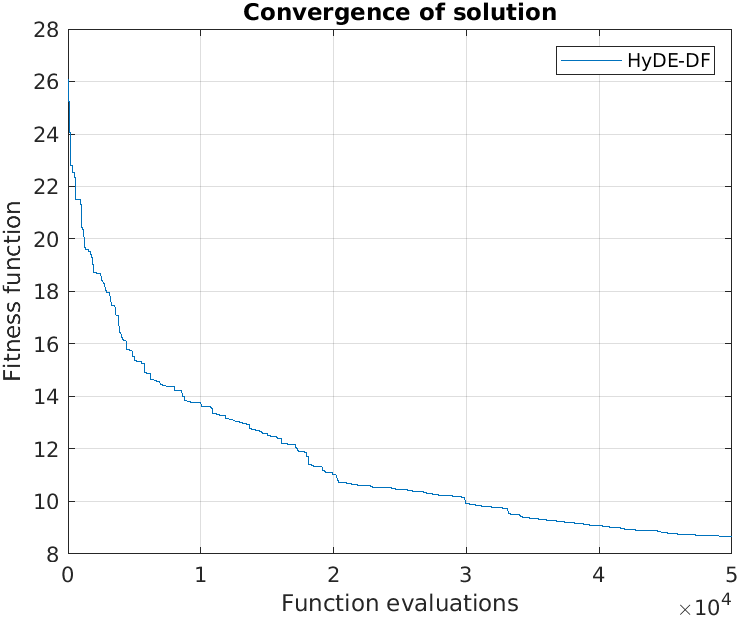
\includegraphics[width=0.5 \textwidth]{images/Examples/HyDE_50000.png}}
    \caption{\label{fig:Model_of_Edge} Вставка одного графика }
    \end{figure}

    Два графика на одном уровне
    \begin{figure}[ht!]
        \centering
        \begin{subfigure}{.5\textwidth}
          \centering
          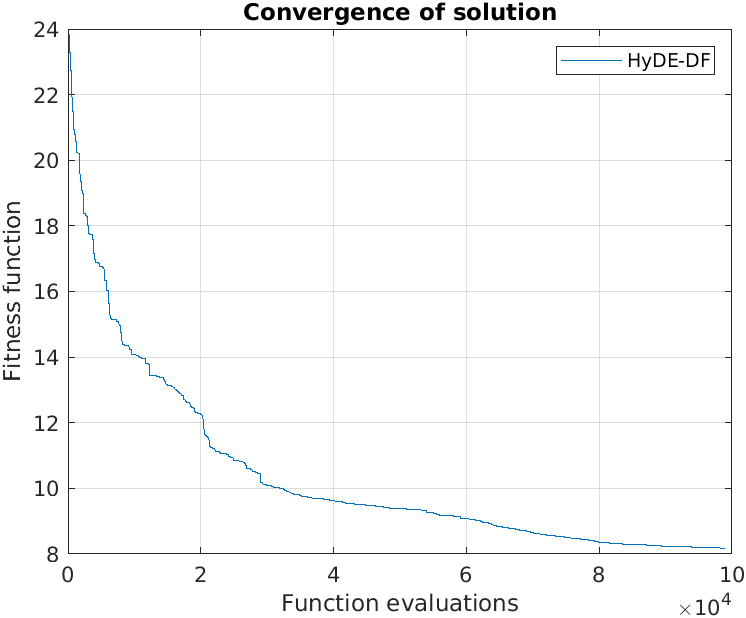
\includegraphics[width=.9\linewidth]{images/Examples/HyDE_100000.png}
          \caption{Левый график}
          \label{fig:sub1}
        \end{subfigure}%
        \begin{subfigure}{.5\textwidth}
          \centering
          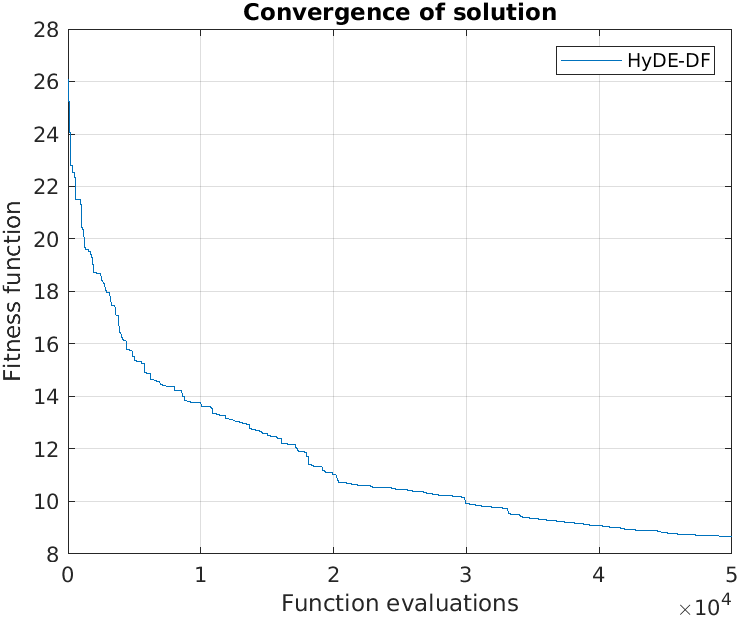
\includegraphics[width=.9\linewidth]{images/Examples/HyDE_50000.png}
          \caption{Правый график}
          \label{fig:sub2}
        \end{subfigure}
        \caption{Вставка двух графиков на одном уровне}
        \label{fig:test}
    \end{figure}
                                     % Вторая глава
\input{5_chap3}                                     % Третья глава
\chapter*{Заключение}
\addcontentsline{toc}{chapter}{Заключение}
    Не хочу вставлять заглушку, поэтому просто напишу, что заключение и выводы это разные штуки, поэтому нужно бы написать и то, и другое, вот.                                  % Заключение

\printbibliography[title=Список использованных источников] 
% Автособираемый список источников

\end{document}